Unlike Lagrange FEs \emph{boundary conditions} (BCs) for $C^1$ FEs can be a bit
tricky to implement. We will demonstrate the difficulty of implementing BCs for
$C^1$ FEs through an example. Consider the \emph{Poisson problem}
\begin{equation}
  \begin{split}
    -\Delta &u = f \quad \text{on } \Omega \\
    &u = 0 \quad \text{on } \partial \Omega
  \end{split}
  \label{eqn:Poisson}
\end{equation}
The weak form of \eqref{eqn:Poisson} is given by
\begin{equation}
  \begin{split}
    \text{Fi}&\text{nd }u \in X := H^1_0(\Omega) \text{ such that} \\
    &(\nabla u, \nabla v) = (f, v) \quad \forall v \in X.
  \end{split}
  \label{eqn:PoissonWeak}
\end{equation}
Thus, for conforming FEs the FE formulation is given by
\begin{equation}
  \begin{split}
    &\text{Find }u^h \in X^h \subset X \text{ such that} \\
    (\nabla &u^h, \nabla v^h) = (f, v^h) \quad \forall v^h \in X^h.
  \end{split}
  \label{eqn:PoissonFE}
\end{equation}
Since $u \in H^1_0(\Omega)$ and $u^h \in X^h \subset H^1_0(\Omega)$ only $C^0$
Lagrange FEs need be used. However, for demonstration purposes lets assume $u^h
\in X^h \subset C^1(\Omega) \subset X$ and therefore Lagrange FEs are no longer
an appropriate choice for our FE discretization.

With Lagrange FEs the most straight forward and usual way to deal with BCs is to
enforce them by explicitly setting the degrees of freedom (DoFs) on the boundary
to zero and reduce the linear system to contain only the internal nodes. This
can be seen graphically in \autoref{fig:ReducedBCs}. One major benefit to
treating BCs in this way is in reducing the size of the linear system that must
be solved, and therefore reducing computational time.
\begin{figure}[h]
	\begin{center}
  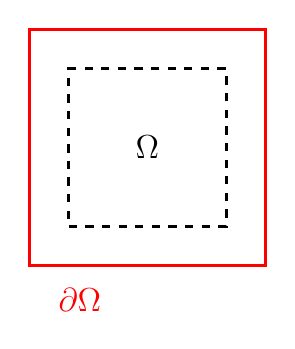
\begin{tikzpicture}[scale=0.5]
    \tikzstyle{every node}=[font=\tiny]
    \draw[style=very thick, color=red] (0,0) node[fill=none, below
      right=1ex,color=red ] { { \large $\partial\Omega$ } } -- (6,0) -- (6,6) --
      (0,6) -- cycle;
    \draw[style=very thick,dashed] (1,1) -- (5,1) -- (5,5) -- (1,5) -- cycle;

    \draw (3,3) node[fill=none] { {\large $\Omega$} };
  \end{tikzpicture}
	\end{center}
  \caption{Eliminated Boundary Nodes}
	\label{fig:ReducedBCs}
\end{figure}


This method can be problematic when using $C^1$ FEs. Consider the boundary
$\partial \Omega = \Gamma_1 \bigcup \Gamma_2$, where $\Gamma_1$ and $\Gamma_2$
correspond to the vertical and horizontal boundaries, respectively (see
\autoref{fig:SplitBoundary}).  On $\Gamma_1$ we know $u=0$ which implies $u_y =
u_{yy} = 0$ on $\Gamma_1$.  While on $\Gamma_2$ we know $u=0$ which implies $u_x
= u_{xx} = 0$ on $\Gamma_2$. Thus, simply setting $u^h = 0$ on the boundary
results in the DoFs corresponding to $u_x,\,u_y,\,u_{xx}$, and $u_{yy}$ not
necessarily being set to zero. Thus, one must force these DoFs to be zero too or
another scheme must be implemented to deal with this case. However, setting the
appropriate DoFs to zero requires some analysis of the problem domain before
implementation, which is problematic when one wants to implement a generalized
code. To avoid this one can implement a Lagrange Multiplier scheme.
\begin{figure}[h]
	\begin{center}
  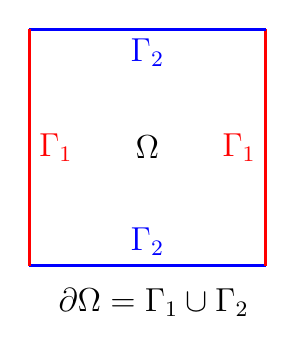
\begin{tikzpicture}[scale=0.5]
    \tikzstyle{every node}=[font=\tiny]
    \draw[style=very thick,color=blue] (0,0)
    node[fill=none, below right=1ex, color=black] { { \large $\partial\Omega = \Gamma_1 \cup \Gamma_2$ } }
    -- (3,0) -- (6,0);
    \draw[style=very thick,color=red] (6,0) -- (6,3) -- (6,6);
    \draw[style=very thick,color=blue] (6,6) -- (3,6) -- (0,6);
    \draw[style=very thick,color=red] (0,6) -- (0,3) -- (0,0);

    \draw (3,3) node[fill=none] { {\large $\Omega$} };
    \draw[color=red] (0,3) node[fill=none,right] { {\large $\Gamma_1$} };
    \draw[color=blue] (3,0) node[fill=none,above] { {\large $\Gamma_2$} };
    \draw[color=red] (6,3) node[fill=none,left] { {\large $\Gamma_1$} };
    \draw[color=blue] (3,6) node[fill=none,below] { {\large $\Gamma_2$} };
  \end{tikzpicture}
	\end{center}
  \caption{Decomposed Boundary}
	\label{fig:SplitBoundary}
\end{figure}


Rewrite the FE formulation, \eqref{eqn:PoissonFE}, in the following way
\begin{equation}
  \begin{split}
    A u &= \ell \\
    \Lambda u &= b,
  \end{split}
  \label{eqn:ConstrainedPoisson}
\end{equation}
where is $\Lambda u = b$ is the constraint equation descibing the boundary
conditions and $A u = \ell$ is the FE formulation of the Poisson equation.
Then the \emph{variational form} of \eqref{eqn:ConstrainedPoisson} is
\begin{equation}
  L(u,\lambda) = \frac{1}{2}u^T A u - u^T \ell + \lambda^T (\Lambda u - b),
  \label{eqn:Variational}
\end{equation}
where $\lambda$ is the Lagrange multiplier. Using the first derivative condition
results in
\begin{equation}
  \begin{split}
    \frac{d L}{du} &= Au - \ell + \Lambda^t \lambda = 0 \\
    \frac{d L}{d\lambda} &= \Lambda u - b = 0.
  \end{split}
  \label{eqn:Condition}
\end{equation}
Thus, given $b = \mathbf{0}$ the new system of equations using Lagrange
multipliers for boundary constraints is given by
\begin{equation}
  \begin{bmatrix}
    A & \Lambda^T \\
    \Lambda &  \mathbf{0} \\
  \end{bmatrix} \begin{bmatrix}
    u \\ \lambda
  \end{bmatrix} = \begin{bmatrix}
    \ell \\ \mathbf{0}
  \end{bmatrix}.
  \label{eqn:Lagrange}
\end{equation}
To avoid zeros on the main diagonal we add a small perturbation, $\varepsilon$,
in the lower right.
